\chapter{Harmonogram realizacji projektu}
\label{cha:harmonogram}

\section{Etapy realizacji oraz wykres Gantta}

Proces tworzenia aplikacji \texttt{YLO GradeBook} został zaplanowany jako ciąg kolejnych etapów, obejmujących m.in. analizę wymagań, projektowanie architektury, tworzenie interfejsu użytkownika, implementację logiki systemu, testowanie oraz przygotowanie dokumentacji technicznej.

Realizacja przebiegała zgodnie z przyjętym harmonogramem, jednak w trakcie realizacji konieczne było kilkukrotne cofnięcie się do wcześniejszych faz projektu — w celu wprowadzenia poprawek lub dostosowania struktury do nowych funkcjonalności.

Warto podkreślić, że wiele zadań prowadzono równolegle, ponieważ dawało to swobodę realizacji nowych pomysłów. 

W celu zobrazowania kolejnych faz projektu, opracowano wykres Gantta (rys. \ref{fig:ganttYLO}) przedstawiający plan pracy.


\begin{figure}[H]
    \centering
    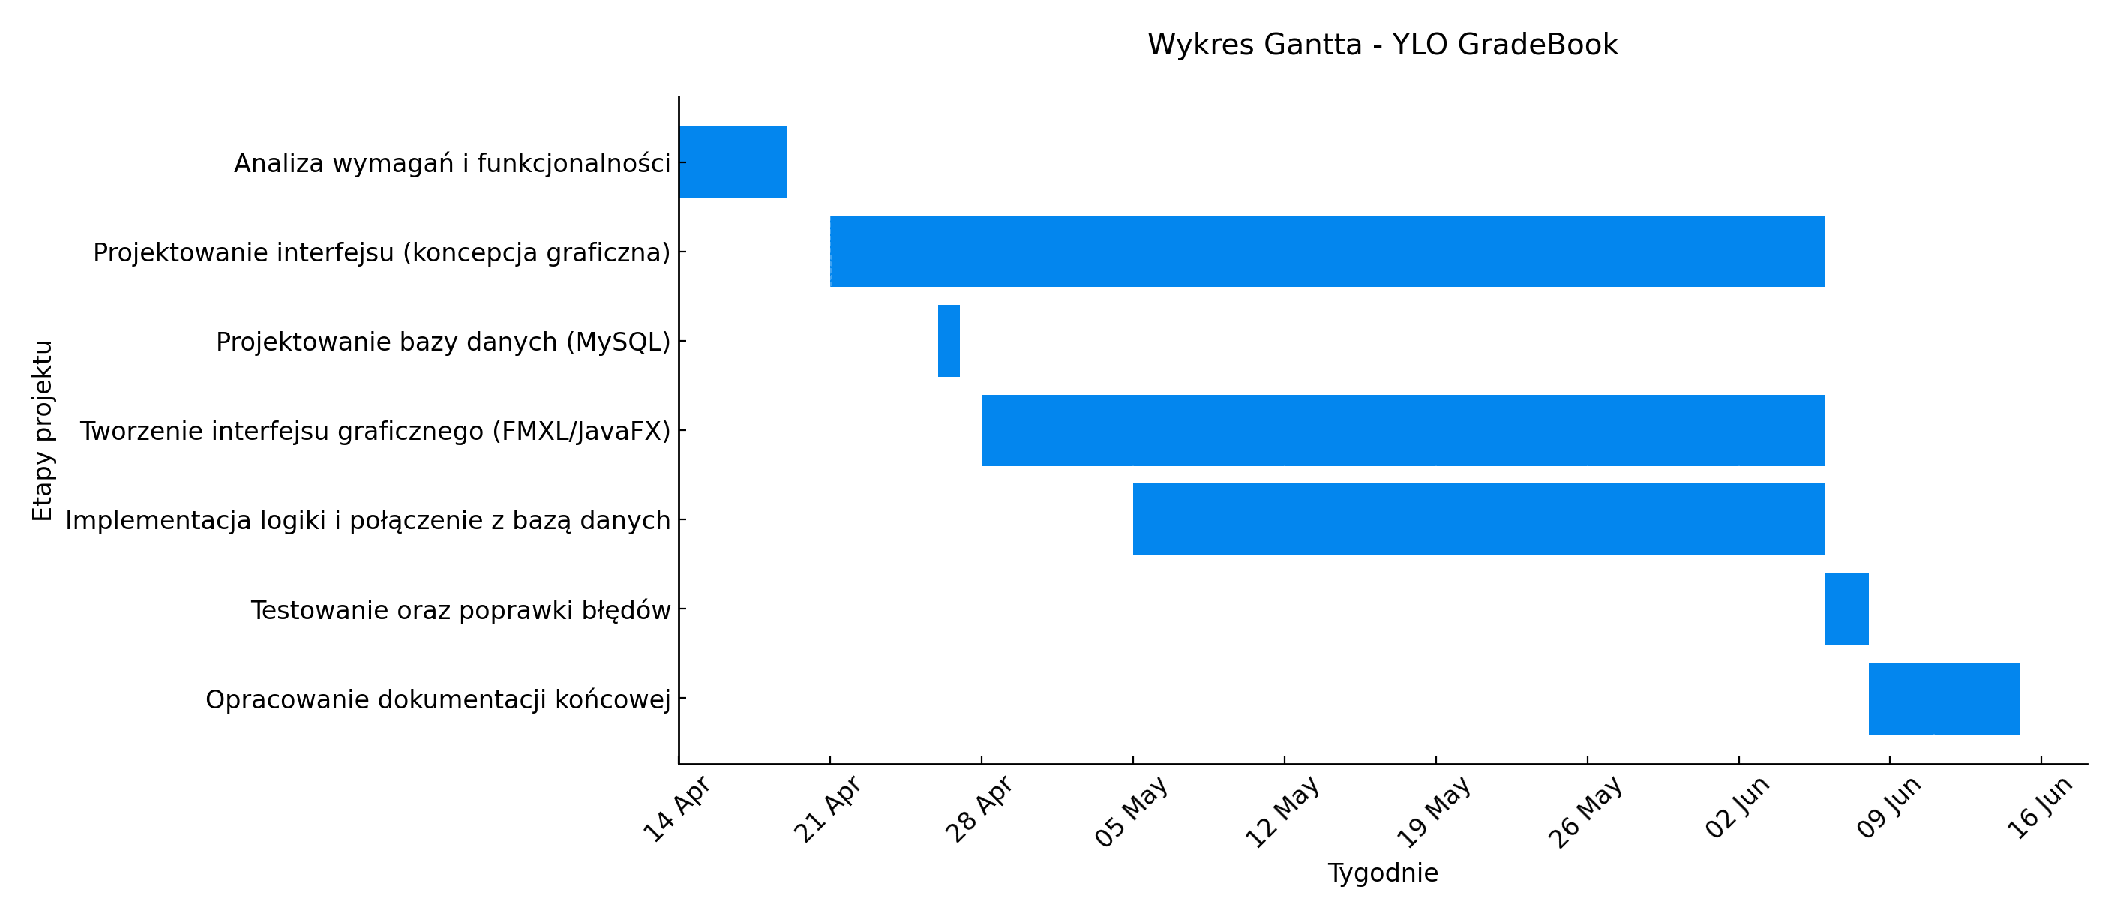
\includegraphics[width=1\textwidth]{figures/fig_0004.eps}
    \caption{Wykres Gantta przedstawiający harmonogram realizacji projektu YLO GradeBook}
    \label{fig:ganttYLO}
\end{figure}

\section{System kontroli wersji i repozytorium projektu}

W trakcie realizacji projektu wykorzystano system kontroli wersji \textbf{Git}, który umożliwił systematyczne zapisywanie kodu.  Do przechowywania i synchronizacji kodu źródłowego użyto platformy \textbf{GitHub}.

Pełne repozytorium projektu \texttt{YLO GradeBook} jest dostępne pod adresem:

\begin{center}
\texttt{https://github.com/oleiy/YLO-GradeBook}
\end{center}

Repozytorium zawiera ostateczną wersję projektu, okumentację projektowa oraz bazę danych. Zgodnie z wymaganiami, projekt dostępny będzie przez cały rok.